\documentclass[
    report,
    11pt,
    oneside,
    a4paper,
    english,
    brazil,
    sumario=tradicional
    ]{abntex2}


% Pacotes fundamentais
\usepackage{lmodern}
\usepackage[T1]{fontenc}
\usepackage[utf8]{inputenc}
\usepackage{indentfirst}
\usepackage{nomencl}
\usepackage{color}
\usepackage{microtype}
\usepackage{graphicx}
\graphicspath{{img/}}

% Pacotes adicionais
\usepackage{lipsum}
\usepackage[brazilian,hyperpageref]{backref}
\usepackage[alf]{abntex2cite}

% Configurações do pacote backref
\renewcommand{\backrefpagesname}{Citado na(s) página(s):~}
\renewcommand{\backref}{}
\renewcommand*{\backrefalt}[4]{
    \ifcase #1
        Nenhuma citação no texto.
    \or
        Citado na página #2.
    \else
        Citado #1 vezes nas páginas #2.
    \fi}%

\title{Os Efeitos Adversos da GDPR}
\tituloestrangeiro{\textbf{How the GDPR Failed} \\ \Large{And how we can still succeed}}

\autor{Pedro Sader Azevedo}
\instituicao{Universidade Estadual de Campinas}
\local{Brasil}

% Configurações de aparência do PDF final
% alterando o aspecto da cor azul
\definecolor{blue}{RGB}{41,5,195}

\makeatletter
\hypersetup{
   pagebackref=true,
   pdftitle={\@title},
   pdfauthor={\@author},
   pdfsubject={A complexidade do problema da desigualdade salarial entre homens e mulheres},
   pdfcreator={LaTeX with abnTeX2},
   pdfkeywords={ods}{gênero}{salário}{ocupação},
   colorlinks=true, % false: boxed links; true: colored links
   linkcolor=blue, % color of internal links
   citecolor=blue, % color of links to bibliography
   filecolor=magenta, % color of file links
   urlcolor=blue,
   bookmarksdepth=4
}
\makeatother

% compila o indice
\makeindex

% margens
\setlrmarginsandblock{3cm}{3cm}{*}
\setulmarginsandblock{3cm}{3cm}{*}
\checkandfixthelayout

% tamanho da indentação
\setlength{\parindent}{1.3cm}

% espaçamento entre parágrafos
\setlength{\parskip}{0.2cm}
% \setlength{\onelineskip}

\SingleSpacing


\begin{document}

\selectlanguage{brazil}

\frenchspacing

\maketitle

\textual

A Regulamentação Geral de Proteção de Dados (GDPR) foi a principal política pública europeia referente à questão da privacidade digital~\cite{gdpr}. Essa lei foi tomada como referência em diversas partes do mundo, inclusive servindo de base para a criação da Lei Geral de Proteção de Dados no Brasil~\cite{lgpd}. No entanto, as medidas estabelecidas pela GDPR provaram-se não apenas ineficazes em ampliar o respeito pelo Direito Humano à privacidade, como também introduziram novos empecilhos a conquista desse direito.

Uma das mais emblemáticas resoluções da GDPR foi a proibição da coleta de dados pessoais sem consentimento explícito~\cite{data-consent}. Apesar de ``bem-intencionada'', essa imposição teve como efeito adverso uma abundância desmedida de \textit{cookie popups}, isto é, mensagens que cobrem o conteúdo de páginas da web até que o usuário ceda a permissão para coleta e processamento de seus dados.

\begin{figure}[h]
    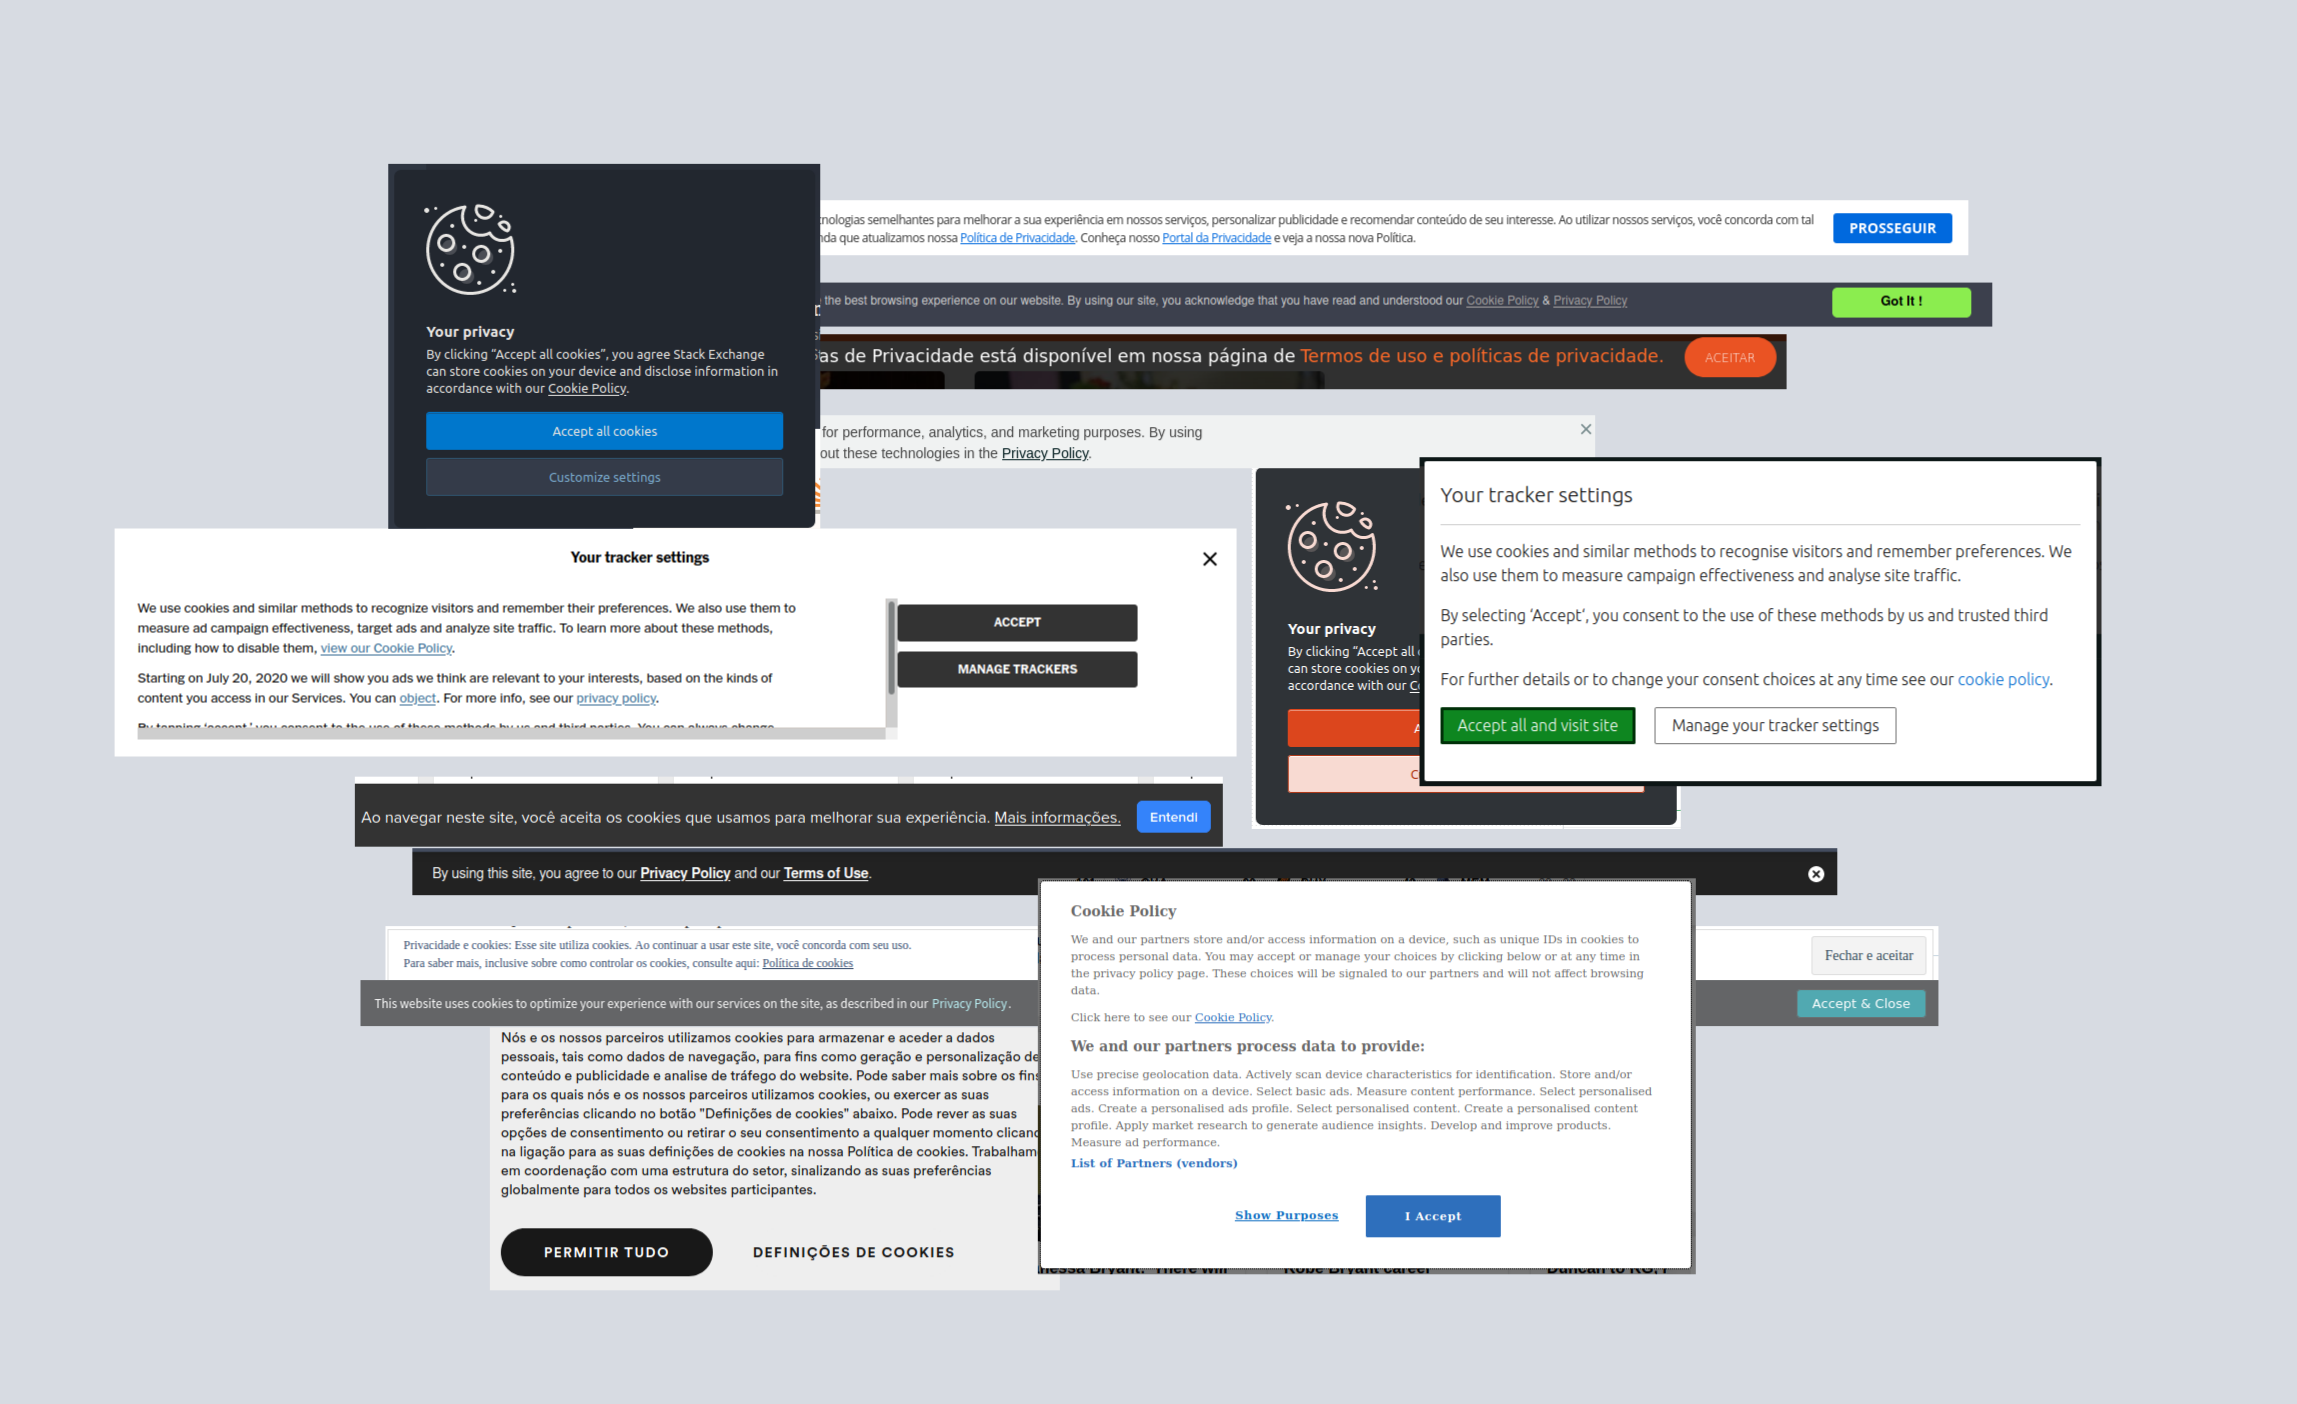
\includegraphics[width=\textwidth]{cookies.png}
    \centering
    \caption{A Internet depois da GDPR (autoral)}
\end{figure}

Consequência imediata disso foi uma queda dramática na qualidade da experiência de usuário, visto que interrupções constantes se tornaram regra (ou melhor, lei), em vez de excessão. Prova desse incômodo, é que extensões de navegador, como a genial \textit{I don't care about cookies}~\cite{i-dont-care-about-cookies}, foram desenvolvidas para remover esse tipo de distração. Ademais, estudos apontam que mencionar ``personalização'' ou ``aprimoramento de serviços'' aumenta significativamente o poder persuasivo dos \textit{cookie banners}~\cite{cookie-strategies}, muitas vezes levando à decisão mal-informada de consentir.

Enfim, por mais que a GDPR não tenha sido perfeita, é inegável sua importância para a questão da privacidade digital. No mínimo, ela desencadeou a tendência de regulamentar mais estritamente os mercado digitais \cite{dma} e, por isso, merece crédito.

\pagebreak

\postextual

\bibliography{ref}

\end{document}
